\documentclass[10.5pt,a4paper]{article}
\usepackage[margin=2.1cm]{geometry}
\usepackage[T1]{fontenc}\usepackage{lmodern}
\usepackage{amsmath,amssymb,booktabs,graphicx,float,caption,array,longtable,adjustbox,enumitem,xcolor}
\usepackage[most]{tcolorbox}
\usepackage{tikz}
\usetikzlibrary{arrows.meta,positioning,calc}
\usepackage[hidelinks]{hyperref}
\usepackage{titlesec}
\titleformat{\section}{\large\bfseries\color{black}}{\thesection}{0.8em}{}
\captionsetup{font=small,labelfont=bf}
\setlength{\parskip}{0.45em}\setlength{\parindent}{0pt}
\definecolor{acc}{HTML}{2a78d6}
\newcommand{\finPR}{16}
\newcommand{\finTITC}{1400}
\newcommand{\finTITK}{1673}
\newcommand{\finX}{0.30}
\newcommand{\finE}{11.9}
\newcommand{\finEps}{0.85}
\newcommand{\finEta}{40.5}
\newcommand{\finEtaTh}{41.1}
\newcommand{\finHR}{8,885}
\newcommand{\finLCOE}{11.34}
\newcommand{\finCO}{0.439}
\newcommand{\finNOx}{29.6}
\newcommand{\finFI}{1.29}
\newcommand{\finXd}{4.43}
\newcommand{\finPsi}{39.4}
\newcommand{\finMair}{237.6}
\newcommand{\finMfuel}{4.78}
\newcommand{\finMh}{0.244}
\newcommand{\finCapex}{534}
\newcommand{\finWnet}{427}
\newcommand{\finCool}{10.3}
\newcommand{\finTfive}{826}
\newcommand{\finTsix}{647}
\newcommand{\finTfour}{879}
\newcommand{\finTtwo}{523}
\newcommand{\finArea}{15,448}
\newcommand{\finQrg}{64.9}
\newcommand{\finStore}{7.0}
\newcommand{\bcEta}{31.4}
\newcommand{\bcLCOE}{10.94}
\newcommand{\bcCO}{0.643}
\newcommand{\bcNOx}{25.0}
\newcommand{\bcCool}{15.0}
\newcommand{\bcXd}{5.19}
\newcommand{\buEta}{34.67}
\newcommand{\buLCOE}{10.03}
\newcommand{\buCO}{0.583}
\newcommand{\ngLCOE}{9.00}
\newcommand{\ngCO}{0.499}
\newcommand{\dCOpct}{32}
\newcommand{\dLpct}{3.7}
\newcommand{\abateTot}{1,967}
\newcommand{\abateHtwo}{39,254}
\newcommand{\abateCycle}{-13,473}
\newcommand{\dCOcyclepct}{22}
\newcommand{\ruEta}{37.9}
\newcommand{\ruLCOE}{12.11}
\newcommand{\ruCO}{0.469}
\newcommand{\ruNOx}{18.4}
\newcommand{\ruXd}{4.61}
\newcommand{\ruPR}{30}
\newcommand{\ruTITC}{1300}
\newcommand{\ruX}{0.30}
\newcommand{\nScan}{13,200}
\newcommand{\nScanFeas}{4,337}
\newcommand{\nFeas}{106,539}
\newcommand{\nPareto}{9,653}
\newcommand{\nDom}{0}
\newcommand{\noxK}{1.31}
\newcommand{\noxN}{1.09}
\newcommand{\lcoeLo}{10.72}
\newcommand{\lcoeHi}{11.78}
\newcommand{\parityPrice}{304}
\newcommand{\fuelShare}{86}

\newcommand{\Rs}{Rs~}

\begin{document}
\begin{titlepage}
\centering
{\large ME 306 -- Course Project Report\par}
\vspace{1.2cm}
{\LARGE\bfseries Hydrogen-Fuelled / Hydrogen-Blended Gas Turbine\\for Decarbonised Grid Power\par}
\vspace{0.6cm}
{\Large Problem 16\par}
\vspace{1.4cm}
{\Large\bfseries Role R5 -- Integration \& Fuel Supply\par}
\vspace{0.4cm}
{\large Integrated cycle model, overall exergy balance, LCOE and CO$_2$,\\ five-objective NSGA-II optimisation and final design selection\par}
\vspace{1.6cm}
\begin{tcolorbox}[colback=acc!6,colframe=acc,width=0.86\textwidth,title=\textbf{Recommended configuration}]
\centering
\textbf{Intercooled + regenerative Brayton cycle (no reheat)}\\[3pt]
Pressure ratio \finPR{} $\cdot$ TIT \finTITC\,\textdegree C $\cdot$ hydrogen \finX{} by volume (\finE\% of fuel energy) $\cdot$ regenerator $\varepsilon=\finEps$\\[3pt]
$\eta_{net}=\finEta\%$ $\cdot$ LCOE \Rs\finLCOE/kWh $\cdot$ \finCO{} kg CO$_2$/kWh $\cdot$ NOx index \finNOx{} ppm
\end{tcolorbox}
\vfill
{\small Builds on the R1 (compressor \& intercooling), R2 (combustor \& fuel blend), R3 (turbine \& reheat) and R4 (regenerator) submissions.\\
All numbers in this report are generated by the accompanying Python code (folder \texttt{R5\_Integration}).\par}
\end{titlepage}

\section*{Summary}
\begin{itemize}[leftmargin=1.2em,itemsep=2pt]
\item \textbf{Integration.} R1--R4 were combined into one constant-$c_p$ cycle model with a shared parameter file and one state numbering. It reproduces the plan's Week-2 reference (721.8\,K, $f=0.0263$, 944.6\,K, 444.1\,kJ/kg, 35.20\%/\buEta\%, \Rs\buLCOE/kWh). It also reproduces every teammate hand-off to the stated digits: R1's two-stage compressor, R4's regenerator duty, area and LCOE, and R2's eight-configuration table. The exergy balance closes to $10^{-13}$\,kJ/kg.
\item \textbf{Blade cooling} is not given in the problem statement. It was added from cited web data: firing limit 1500\,\textdegree C (G/H-class air-cooled technology), blade-metal limit 1150\,K, and coolant calibrated to 15\% of compressor air at 1400\,\textdegree C. With cooling, the natural-gas baseline drops from 34.7\% to \bcEta\%. Reheat loses most, because its second turbine must also be cooled. Intercooling gains, because colder compressor delivery means less coolant.
\item \textbf{Optimisation.} NSGA-II was run on each of the 8 on/off configurations, over pressure ratio, TIT, hydrogen share and regenerator effectiveness, with 5 objectives and 6 constraints. Together with a \nScan-point grid scan, this gave \nFeas{} feasible designs and a 5-objective Pareto set of \nPareto{} designs.
\item \textbf{Selection.} TOPSIS was run with two normalisations and five weight sets. The two equal-weight winners were then compared directly. The intercooled + regenerative design is better on 4 of the 5 objectives (efficiency, exergy destruction, LCOE, CO$_2$). Its NOx index is \finNOx{} ppm, 40\% of the 75\,ppm CPCB limit, and it needs no reheat combustor, which avoids that combustor's hydrogen autoignition risk.
\item \textbf{Outcome vs.\ the cooled natural-gas baseline:} efficiency \bcEta\%\,$\rightarrow$\,\finEta\%, CO$_2$ $-\dCOpct$\% (\bcCO\,$\rightarrow$\,\finCO{} kg/kWh), LCOE $+\dLpct$\% (\Rs\bcLCOE\,$\rightarrow$\,\Rs\finLCOE/kWh). The cycle changes cut CO$_2$ by \dCOcyclepct\% while \emph{saving} money. The 30\% hydrogen blend costs about \Rs\abateHtwo{} per tonne of CO$_2$ avoided. At hydrogen prices below about \Rs\parityPrice/kg, the final design is cheaper than the cooled baseline.
\end{itemize}

\tableofcontents
\newpage

%=====================================================================
\section{R5 scope and deliverables}
The problem statement gives R5 the job of assembling R1--R4 into complete candidate configurations. R5 computes net work, efficiency, heat rate and the air and fuel flows for 100\,MW. It builds the overall exergy balance and the second-law efficiency, and computes the LCOE (including hydrogen supply and storage) and the CO$_2$ per kWh. R5 also runs the multi-objective optimisation and selects one design. Table~\ref{tab:scope} maps each requirement to where it is answered.

\begin{table}[H]\centering\small\caption{R5 requirements (problem statement \S3--4 and the four-week plan) and where they are answered.}\label{tab:scope}
\begin{tabular}{p{7.6cm}p{6.6cm}}\toprule Requirement & Where \\\midrule
Shared parameter file, state numbering, assumptions log & \S\ref{sec:recon}, \S\ref{sec:model}, Appendix A; \texttt{r5\_params.py}\\
Integrated baseline matches the plan's reference numbers & \S\ref{sec:valid}, Table~\ref{tab:valid}\\
Net work, efficiency, heat rate, air and fuel flow for 100\,MW & \S\ref{sec:cand}, \S\ref{sec:final}, Table~\ref{tab:perf}\\
Overall exergy balance and second-law efficiency & \S\ref{sec:exergy}, Table~\ref{tab:exergy}\\
LCOE incl.\ hydrogen supply and storage; CO$_2$ per kWh & \S\ref{sec:model}, \S\ref{sec:final}, Tables~\ref{tab:capex}--\ref{tab:lcoe}\\
Variables, objectives, constraints; NSGA-II across 5 objectives & \S\ref{sec:moo}\\
Feasible set after constraint filtering; Pareto plots (4 pairs) & \S\ref{sec:moo}, Fig.~\ref{fig:pareto}\\
TOPSIS / reasoned trade-off; final design and justification & \S\ref{sec:select}, \S\ref{sec:final}\\
What the final design gives up against each role's best & \S\ref{sec:roles}\\
Robustness and sensitivity runs & \S\ref{sec:sens}\\\bottomrule
\end{tabular}\end{table}

%=====================================================================
\section{Inputs from R1--R4 and reconciliation}\label{sec:recon}
Each teammate's module was taken as submitted. Where submissions disagreed, R5 fixed one value for the whole team (Table~\ref{tab:recon}).

\begin{table}[H]\centering\small\caption{Inconsistencies found across the R1--R4 submissions and the value R5 adopted.}\label{tab:recon}
\begin{tabular}{p{3.2cm}p{6.2cm}p{5.6cm}}\toprule Item & Finding & R5 decision \\\midrule
Hydrogen-share basis & R2: volume (mole) fraction, with energy share from mass-basis LHV (11.9\% at $x=0.3$). R4: volumetric LHVs (11.45\%) & Volume fraction $x$ everywhere; energy share by R2's method\\
Intercooler $\varepsilon$ & R1 candidate 0.85; R2's stand-in used 0.90 & 0.85 (R1 owns it); 2\% intercooler pressure loss (R1 neglected it)\\
Regenerator $\varepsilon$ & R4 0.75 (range 0.50--0.85); R2's stand-in used 0.70 & Decision variable, 0.50--0.85; 2\% loss per side (R4's 1--3\% range)\\
Regenerator cost & R4: 8--12\% of base; R2: 8\% flat & Proportional to $UA$, calibrated to R4 (Rs 40 cr at $UA=576$\,kW/K). This reproduces 8\% at $\varepsilon=0.70$ and 12.7\% at 0.80\\
Air mass flow & R1 used 230.2\,kg/s (R4's regenerated case) & Re-sized for every design: $\dot m_a=100\,\text{MW}/(\eta_g w_{net})$\\
Firing limit and blade cooling & R3 report: ``not supplied''. R3 code assumed 1500\,\textdegree C, 1150\,K metal, about 12\% coolant. R2's stand-in had no cooling & Cooling included in all optimisation runs, with cited parameters (\S\ref{sec:cool}). The baseline is validated uncooled\\
Reheat layout & R2: equal pressure split, reheat to TIT. R3 optimised the split & R2's split (R2's autoignition limits were derived for it); reheat to TIT\\
Reheat-combustor H$_2$ & R2 limit $x\le0.27/0.41/0.47$ at PR 10/15/20 & Interpolated in PR, held constant outside 10--20\\
Exergy as an objective & Plan: confirm with instructor; problem statement lists it as Objective 2 & Included as Objective 2 (MJ destroyed per kWh)\\
CPCB NOx limit & 75\,ppm from a secondary source (R2) & 75\,ppm used, flagged for gazette verification; 50\,ppm used as a stricter check\\
H$_2$ storage cost & Problem statement: team to find & R2's figure: Rs 55,000/kg capacity, 8 h at full load (US DOE)\\
R2 stand-in selection & IC+Regen+Reheat, PR 15, $x=0.40$, from a 216-point grid without cooling & Superseded by the NSGA-II run here; re-evaluated in \S\ref{sec:roles}\\\bottomrule
\end{tabular}\end{table}

%=====================================================================
\section{Integrated cycle model}\label{sec:model}
\subsection{Plant and state numbering}
Figure~\ref{fig:schem} shows the team's master schematic. Every optional block is a separate on/off case: intercooler (R1), regenerator (R4), and reheat combustor plus LP turbine (R3). All specific quantities are per kg of compressor-inlet air, with $h=c_pT$ as in the plan.

\begin{figure}[H]\centering
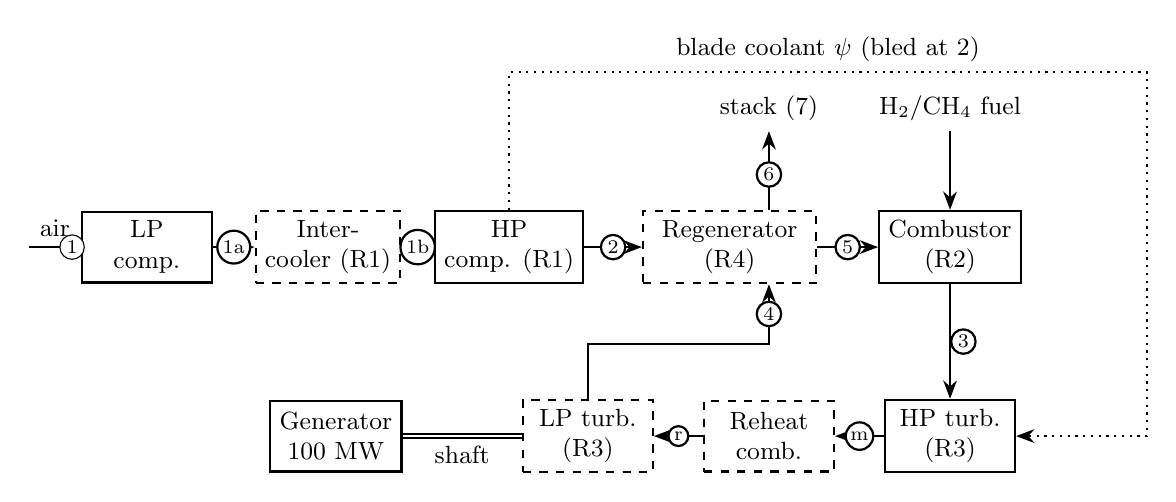
\begin{tikzpicture}[font=\small,>=Stealth,box/.style={draw,thick,minimum width=1.65cm,minimum height=0.9cm,align=center},opt/.style={box,dashed},st/.style={circle,fill=white,draw,inner sep=1pt,font=\scriptsize}]
\node[box] (lpc) at (0,0) {LP\\comp.};
\node[opt] (ic) at (2.3,0) {Inter-\\cooler (R1)};
\node[box] (hpc) at (4.6,0) {HP\\comp. (R1)};
\node[opt,minimum width=2.2cm] (rg) at (7.4,0) {Regenerator\\(R4)};
\node[box] (cc) at (10.2,0) {Combustor\\(R2)};
\node[box] (hpt) at (10.2,-2.4) {HP turb.\\(R3)};
\node[opt] (rh) at (7.9,-2.4) {Reheat\\comb.};
\node[opt] (lpt) at (5.6,-2.4) {LP turb.\\(R3)};
\node[box] (gen) at (2.4,-2.4) {Generator\\100 MW};
\draw[->,thick] (-1.5,0) -- node[above]{air} (lpc);
\draw[->,thick] (lpc) -- node[st,pos=0.5]{1a} (ic);
\draw[->,thick] (ic) -- node[st,pos=0.5]{1b} (hpc);
\draw[->,thick] (hpc) -- node[st,pos=0.5]{2} (rg);
\draw[->,thick] (rg) -- node[st,pos=0.5]{5} (cc);
\draw[->,thick] (cc) -- node[st,right]{3} (hpt);
\draw[->,thick] (hpt) -- node[st,pos=0.5]{m} (rh);
\draw[->,thick] (rh) -- node[st,pos=0.5]{r} (lpt);
\draw[->,thick] (lpt.north) -- ++(0,0.7) -| node[st,pos=0.75]{4} ($(rg.south)+(0.5,0)$);
\draw[->,thick] ($(rg.north)+(0.5,0)$) -- node[st,pos=0.45]{6} ++(0,1.0) node[above]{stack (7)};
\draw[->,thick] ($(cc.north)+(0,1.0)$) node[above]{H$_2$/CH$_4$ fuel} -- (cc.north);
\draw[->,dotted,thick] (hpc.north) -- ++(0,1.75) -- ++(8.1,0) node[pos=0.5,above]{blade coolant $\psi$ (bled at 2)} |- (hpt.east);
\node[st] at (-0.95,0) {1};
\draw[thick,double] (gen) -- node[below]{shaft} (lpt);
\end{tikzpicture}
\caption{Integrated plant (dashed = optional block, each combination run as its own case). Without reheat, the HP turbine expands directly to state 4. Without regeneration, $5\equiv2$ and $6\equiv4$.}\label{fig:schem}
\end{figure}

\subsection{Module equations}
\textbf{Compression (R1).} $p_1=0.99p_0$, $p_2=r_pp_1$. Single stage: $T_2=T_1[1+(r_p^{k_a}-1)/\eta_c]$ with $k_a=(\gamma_a-1)/\gamma_a$. Intercooled: equal stage ratios $r_s=\sqrt{r_p/(1-\delta_{IC})}$, $T_{1b}=T_{1a}-\varepsilon_{IC}(T_{1a}-T_0)$, and $w_c=c_{p,a}[(T_{1a}-T_1)+(T_2-T_{1b})]$.

\textbf{Combustor (R2).} Hand energy balance (as in R2, R4 and the plan) per kg of combustor air: $f_1=(c_{p,g}T_3-c_{p,a}T_5)/(\eta_bLHV_{bl}-c_{p,g}T_3)$. Here $LHV_{bl}=(1-y)48+120y$\,MJ/kg, where $y$ is the H$_2$ mass share obtained from $x$. The hot-gas $c_{p,g}(x)$ and $\gamma_g(x)$ come from R2's Cantera table (1.150$\to$1.191\,kJ/kg\,K and 1.3330$\to$1.3374), so that natural gas reproduces the plan's values exactly. The reheat combustor uses the same balance, from the HP-turbine exit to TIT.

\textbf{Turbines and cooling (R3).} The turbines use the polytropic efficiency equivalent to $\eta_t=0.90$ over each expansion ratio. This keeps the overall efficiency unchanged when an expansion is split at the coolant-injection point. Coolant $\psi$ (per kg of compressor air) is bled at state 2 and mixed in at the mid log-pressure of each turbine, as in R3's code. Combustor air is $a=1-\psi$.

\textbf{Regenerator (R4).} $C_c=a\,c_{p,a}$, $C_h=\dot m_{ex}c_{p,g}$, $\dot Q=\varepsilon C_{min}(T_4-T_2)$, $T_5=T_2+\dot Q/C_c$, $T_6=T_4-\dot Q/C_h$. $UA=NTU\cdot C_{min}$ with the counterflow $NTU(\varepsilon,C_r)$ relation. The coupling of regenerator, combustor and turbine is solved by fixed-point iteration on $T_4$ to $10^{-7}$\,K.

\textbf{Plant.} $w_{net}=w_t-w_c$, $\eta_{th}=w_{net}/(f_{tot}LHV)$, $\eta_{net}=\eta_g\eta_{th}$, heat rate $=3600/\eta_{net}$, $\dot m_a=100\,000/(\eta_gw_{net})$, $\dot m_f=f_{tot}\dot m_a$, $\dot m_{H_2}=y\dot m_f$.

\subsection{Blade cooling and firing limit (web data)}\label{sec:cool}
The problem statement asks that TIT stay within the firing limit of an \emph{assumed} hot-section technology, but gives no number. The values below were taken from published sources.
\begin{itemize}[leftmargin=1.2em,itemsep=1pt]
\item \textbf{Firing-temperature limit 1500\,\textdegree C (1773\,K).} Mitsubishi lists its F-series at the 1400\,\textdegree C class and its G/H-series at the 1500\,\textdegree C class. Only the J-series reached 1600\,\textdegree C, and it uses steam cooling of stationary parts [W1,W2]. The baseline 1400\,\textdegree C therefore corresponds to F-class. 1500\,\textdegree C is taken as the limit of established air-cooled technology, and TIT is searched over 1300--1500\,\textdegree C.
\item \textbf{Allowable blade-metal temperature 1150\,K (R3's value).} At a 1400\,\textdegree C entry, the coated blade surface runs near 1100\,\textdegree C and the metal about 930\,\textdegree C (1203\,K) [W3]. CMSX-4 single-crystal blades have been flight-qualified at metal temperatures approaching 1130\,\textdegree C [W4]. A lower 1150\,K is kept because a 25-year base-load industrial life needs more margin than an aero engine.
\item \textbf{Coolant flow.} R3's Horlock-type relation: $\phi=(T_3-T_m)/(T_3-T_2)$, $\varepsilon_c=\phi/[\eta_{cool}(1-\phi)]$, $\psi=B(c_{p,g}/c_{p,a})\varepsilon_c\,h_x$, with $\eta_{cool}=0.70$. The blade heat-transfer index $h_x$ rises from 1.000 to 1.034 as $x$ goes from 0 to 1 (R3, Dittus--Boelter, Cantera properties). This captures the higher water content of hydrogen exhaust. $B=0.075$ gives $\psi=15\%$ at 1400\,\textdegree C. This lies between R3's 12\% and the roughly 20\% of compressor air quoted for 1350\,\textdegree C-class industrial machines, which includes sealing air [W5]. Aero engines take 20--25\% [W6]. The sensitivity covers 10--20\%.
\end{itemize}

\subsection{Constraint indicators (from R2)}
\begin{itemize}[leftmargin=1.2em,itemsep=1pt]
\item \textbf{NOx index.} R2's calibrated Zeldovich index (25\,ppm at a 1790\,K primary zone on natural gas), with R2's re-tuned-burner hydrogen factor (1.00 at $x=0$ up to 1.384 at $x=1$). Raising TIT above 1400\,\textdegree C keeps R2's dilution margin, so $T_{pz}=1790+(T_3-1673)$\,K, and NOx follows R2's $T_{pz}$ table. The effect of combustor-inlet temperature and of reheat dilution was fitted to R2's eight-configuration table: NOx $\propto e^{k(T_5-722)}(f_1/f_{tot})^n$, with $k=\noxK\times10^{-3}$\,K$^{-1}$ and $n=\noxN$. The fit reproduces all eight of R2's values within 0.4\,ppm (Table~\ref{tab:valid} code output).
\item \textbf{Flashback index} $FI(x,T_5)$. R2's tables at 722\,K and 877\,K, interpolated (log) in $x$ and linearly in $T_5$. The limit is $FI\le2.0$, the top of R2's tier-B advanced premixer.
\item \textbf{Autoignition.} Combustor inlet $T_5\le1050$\,K (premixer). Reheat combustor $x\le x_{max}(r_p)$ (R2).
\item \textbf{Regenerator.} Allowed only if $T_4>T_2$, with both terminal approaches $\ge20$\,K (R4).
\end{itemize}

\subsection{Exergy, cost and CO$_2$}
Flow exergy uses constant properties, $\psi=c_p(T-T_0)-T_0[c_p\ln(T/T_0)-R\ln(p/p_0)]$. The dead state is 308.15\,K and 1.013\,bar. Fuel exergy uses R2's Szargut ratios (1.0366 for natural gas, 0.9764 for H$_2$). The destruction in each component is taken from its own exergy balance, so the plant balance $\dot X_{fuel}=\dot W_{el}+\sum\dot X_D+\dot X_{stack}$ closes exactly. The combustor term includes the chemical exergy of the products, which the constant-$c_p$ bookkeeping does not track separately. The second-law efficiency is $\Psi=\dot W_{el}/\dot X_{fuel}$.

LCOE follows the problem statement's worked method: CRF $=0.1018$ (9\%, 25 years), O\&M 3\% of capital, load factor 50\%, natural gas \Rs850/GJ, H$_2$ \Rs350/kg (\Rs2917/GJ). The blend price is energy-weighted. Capital cost = \Rs400 crore base + intercooler 6.5\% + regenerator $\propto UA$ + reheat 12.5\% + R2's H$_2$ combustor premium (0, 4, 15\% of base at $x$ = 0, 0.3, 1) + R3's hot-section premium (+4\% per 100\,K above 1400\,\textdegree C) + \textbf{hydrogen storage}. Storage is sized for 8 hours of full-load H$_2$ flow at \Rs55,000 per kg of capacity (R2, from US DOE data). \textbf{Hydrogen supply} cost is carried in the delivered green-H$_2$ price. Direct CO$_2$ $=3.6/\eta_{net}\times(1-e)\times56.1$\,g/MJ, where $e$ is the H$_2$ energy share. Upstream CO$_2$ of the hydrogen is taken as zero (green H$_2$).

%=====================================================================
\section{Validation against the plan and against R1--R4}\label{sec:valid}
\begin{table}[H]\centering\small\caption{Validation. Each teammate check runs the integrated code with that teammate's own settings: no cooling, no added exchanger losses, and R2's $\varepsilon_{IC}=0.9$ and $\varepsilon_{rg}=0.7$ for R2's table.}\label{tab:valid}
\begin{tabular}{llrr}\toprule Check & Quantity & Reference & R5 model\\\midrule
Plan baseline & Compressor exit T2 (K) & 722 & 721.8\\
 & Fuel-air ratio & 0.026 & 0.0263\\
 & Turbine exit T4 (K) & 944 & 944.6\\
 & Net work (kJ/kg air) & 444 & 444.1\\
 & Cycle efficiency (\%) & 35.2 & 35.2\\
 & Net efficiency (\%) & 34.7 & 34.67\\
 & Heat rate (kJ/kWh) & 10,380 & 10384.0\\
 & Air flow (kg/s) & 229 & 228.6\\
 & Fuel flow (kg/s) & 6.0 & 6.01\\
 & Direct CO$_2$ (kg/kWh) & 0.58 & 0.583\\
 & LCOE (Rs/kWh) & 10.03 & 10.03\\
 & Exergy closure (kJ/kg air) & 0 & -1.7e-13\\
\addlinespace
R1 handoff & LPC exit T (K) & 475.46 & 475.46\\
 & Intercooler exit T (K) & 333.25 & 333.25\\
 & Compressor exit T (K) & 514.18 & 514.18\\
 & Compressor work (kJ/kg) & 349.98 & 349.98\\
\addlinespace
R4 handoff & Air after regenerator T5 (K) & 888.84 & 888.84\\
 & Exhaust after regenerator T6 (K) & 801.76 & 801.76\\
 & Heat recovered (MW) & 38.65 & 38.65\\
 & Net efficiency (\%) & 40.03 & 40.03\\
 & Fuel flow (kg/s) & 5.204 & 5.204\\
 & UA (kW/K) & 576.05 & 576.0\\
 & Regenerator exergy destruction (MW) & 1.172 & 1.172\\
 & LCOE (Rs/kWh) & 8.968 & 8.968\\
\addlinespace
R3 handoff & Coolant fraction (-) & 0.1187 & 0.1198\\
 & Turbine exit T (K) & 887.4 & 889.4\\
 & Net efficiency (\%) & 32.35 & 32.17\\
\addlinespace
R2 config table & Simple net efficiency (\%) & 34.7 & 34.7\\
 & Regen net efficiency (\%) & 39.6 & 39.6\\
 & Reheat net efficiency (\%) & 31.9 & 31.9\\
 & Regen+Reheat net efficiency (\%) & 40.5 & 40.5\\
 & IC net efficiency (\%) & 34.2 & 34.2\\
 & IC+Regen net efficiency (\%) & 43.3 & 43.3\\
 & IC+Reheat net efficiency (\%) & 31.8 & 31.8\\
 & IC+Regen+Reheat net efficiency (\%) & 43.4 & 43.4\\
\bottomrule\end{tabular}
\end{table}
All reference values are matched. The only difference is R3's cooled case (32.17\% against 32.35\%), because R3 rescales gas properties with the fuel-air ratio through Cantera, which the plan's constant-$c_p$ model does not do.

%=====================================================================
\section{Candidate configurations}\label{sec:cand}
Table~\ref{tab:cand} and Fig.~\ref{fig:cand} evaluate all eight combinations at the problem statement's operating point (PR 15, TIT 1400\,\textdegree C) with $x=0.30$ and $\varepsilon_{rg}=0.75$, with and without blade cooling.
\begin{table}[H]\centering\scriptsize\caption{Eight candidate configurations, PR 15, TIT 1400\,\textdegree C, $x=0.30$, $\varepsilon=0.75$. CO$_2$ in kg/kWh, NOx in ppm.}\label{tab:cand}
\adjustbox{max width=\textwidth}{\begin{tabular}{lrrrrrrrrl}\toprule
 & \multicolumn{2}{c}{$\eta_{net}$ (\%)} & \multicolumn{2}{c}{LCOE (Rs/kWh)} & \multicolumn{5}{c}{With cooling}\\
\cmidrule(lr){2-3}\cmidrule(lr){4-5}\cmidrule(lr){6-10}
Configuration & uncooled & cooled & uncooled & cooled & CO$_2$ & NOx & $\psi_{cool}$ & $\Psi$ (\%) & Feasible?\\\midrule
Simple & 34.8 & 31.5 & 12.73 & 13.91 & 0.565 & 25.8 & 0.150 & 30.6 & yes\\
Reheat & 32.0 & 26.0 & 13.88 & 16.73 & 0.684 & 15.0 & 0.301 & 25.3 & yes\\
Regen & 39.5 & 34.0 & 11.48 & 13.11 & 0.524 & 30.2 & 0.150 & 33.0 & yes\\
Regen+Reheat & 40.8 & 30.1 & 11.28 & 14.73 & 0.591 & 19.9 & 0.301 & 29.3 & yes\\
IC & 34.1 & 32.4 & 13.05 & 13.66 & 0.550 & 19.7 & 0.102 & 31.4 & yes\\
IC+Reheat & 31.8 & 28.5 & 14.04 & 15.48 & 0.624 & 12.8 & 0.203 & 27.7 & yes\\
IC+Regen & 43.1 & 39.3 & 10.70 & 11.59 & 0.453 & 28.5 & 0.102 & 38.1 & yes\\
IC+Regen+Reheat & 43.6 & 36.2 & 10.71 & 12.59 & 0.492 & 20.6 & 0.203 & 35.1 & yes\\
\bottomrule\end{tabular}}
\end{table}
\begin{figure}[H]\centering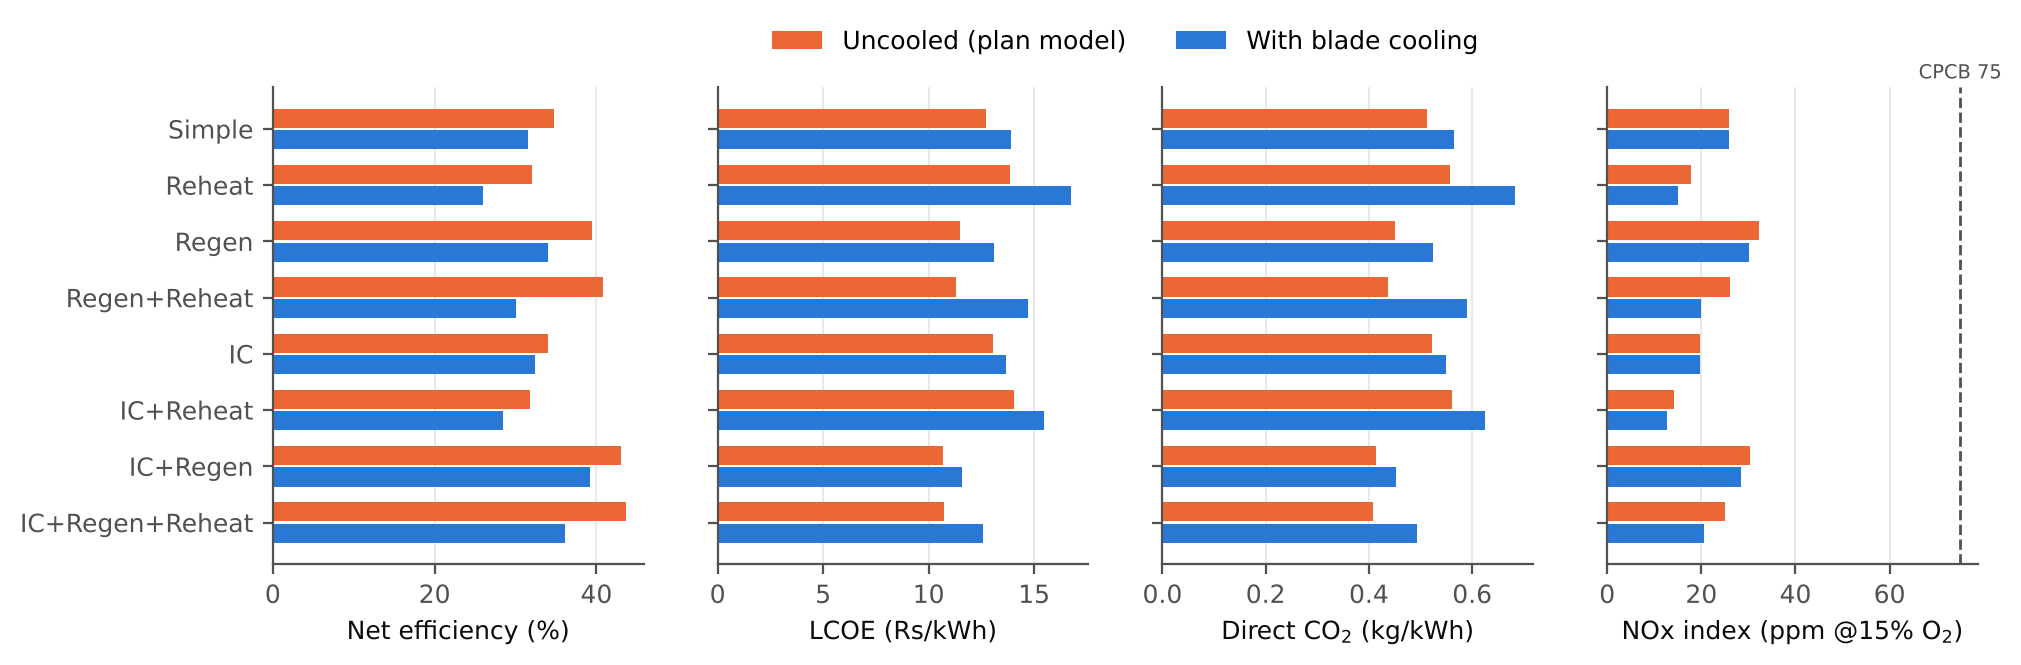
\includegraphics[width=\textwidth]{../figures/fig_candidate_configs.png}
\caption{Candidate configurations, uncooled plan model against the cooled integrated model.}\label{fig:cand}\end{figure}

\textbf{What integration changes.}
\begin{itemize}[leftmargin=1.2em,itemsep=1pt]
\item \textbf{Blade cooling costs about 3 points of efficiency at the baseline.} 15\% of the compressor air bypasses the combustor and is mixed back into the expanding gas. R3's own code showed the same penalty.
\item \textbf{Reheat is penalised most.} The LP turbine is also fired to TIT, so it needs its own coolant (30\% in total at PR 15). Cooled reheat cycles fall below their non-reheat counterparts. R2's uncooled conclusion that IC+Regen+Reheat is best therefore does not survive integration with R3's cooling.
\item \textbf{Intercooling is worth more than R1's compressor-only view suggests.} A colder compressor delivery (516\,K against 722\,K) cuts the coolant requirement from 15\% to 10\%. Together with the larger regeneration margin, IC+Regen is the most efficient cooled layout.
\end{itemize}

\begin{figure}[H]\centering
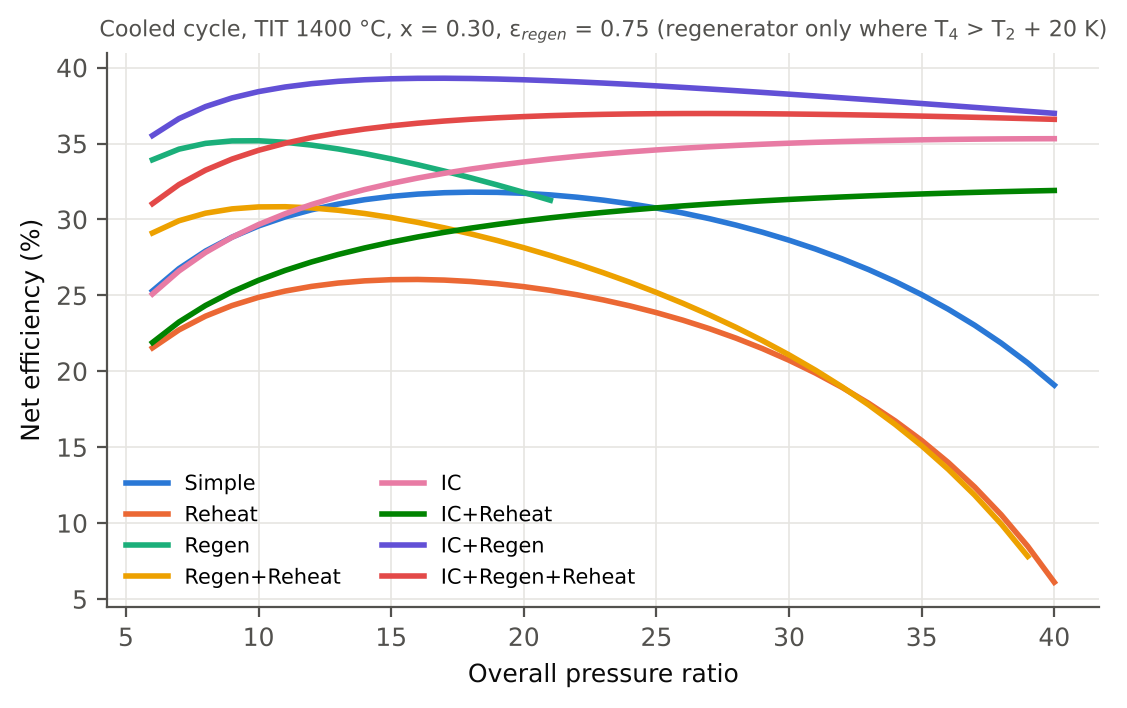
\includegraphics[width=0.62\textwidth]{../figures/fig_pr_sweep.png}
\caption{Efficiency against pressure ratio for each layout (cooled). Regenerative curves stop where $T_4-T_2<20$\,K.}\label{fig:pr}\end{figure}
\begin{figure}[H]\centering
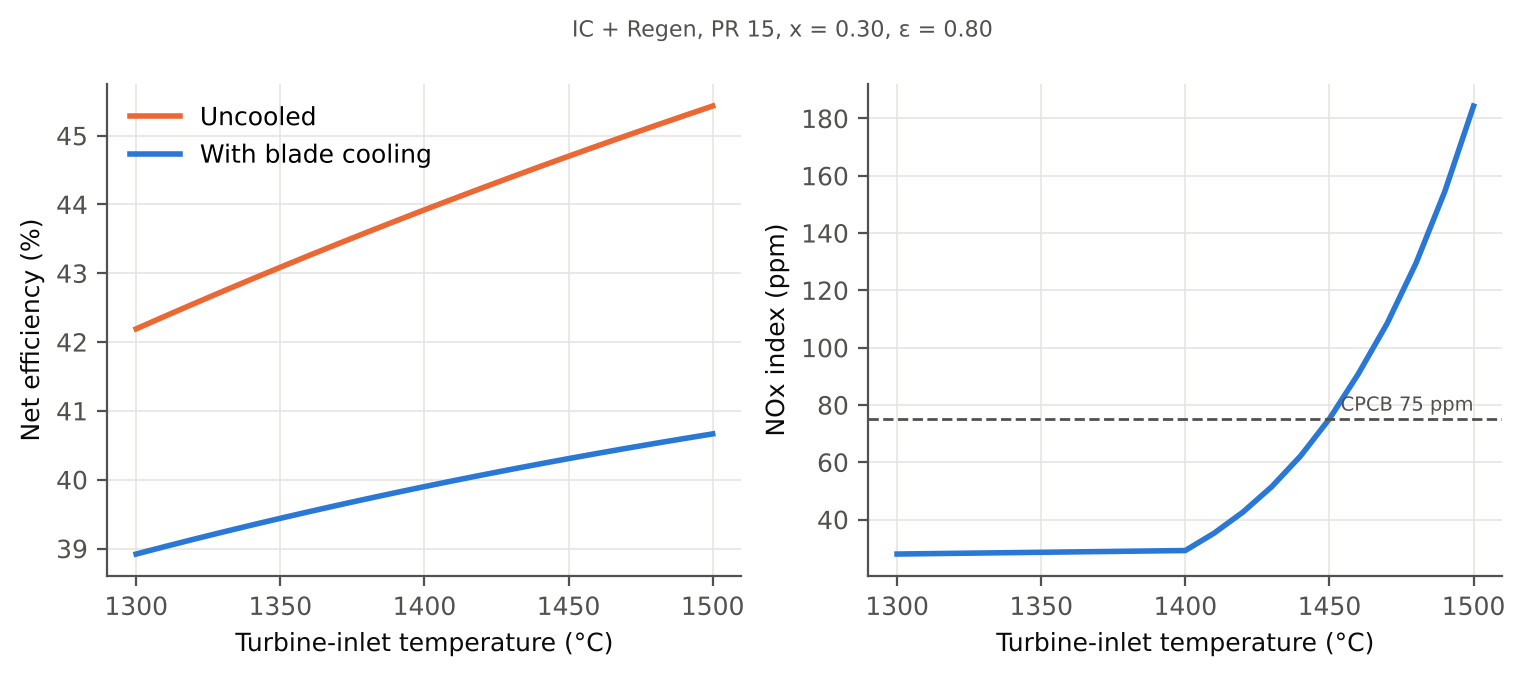
\includegraphics[width=0.85\textwidth]{../figures/fig_tit_tradeoff.png}
\caption{Raising TIT gains only about 0.9 points per 100\,K with cooling (against 1.6 points uncooled). Above about 1450\,\textdegree C the hotter primary zone pushes the NOx index past the CPCB limit, so in practice NOx, not the material, caps TIT.}\label{fig:tit}\end{figure}

%=====================================================================
\section{Overall exergy balance and second-law efficiency}\label{sec:exergy}
\begin{table}[H]\centering\scriptsize\caption{Plant exergy balance at 100\,MW net (MW and \% of fuel exergy). The combustor term includes the chemical exergy of the products.}\label{tab:exergy}
\adjustbox{max width=\textwidth}{\begin{tabular}{lrrrrrr}\toprule
 & \multicolumn{2}{c}{NG baseline (uncooled, reference)} & \multicolumn{2}{c}{NG baseline (cooled)} & \multicolumn{2}{c}{R5 final design}\\
\cmidrule(lr){2-3}\cmidrule(lr){4-5}\cmidrule(lr){6-7}
Item & MW & \% & MW & \% & MW & \%\\\midrule
fuel exergy in & 299.01 & 100.0 & 329.80 & 100.0 & 254.08 & 100.0\\
net electricity & 100.00 & 33.4 & 100.00 & 30.3 & 100.00 & 39.4\\
\midrule
combustor & 105.57 & 35.3 & 116.44 & 35.3 & 86.80 & 34.2\\
reheat combustor & 0.00 & 0.0 & 0.00 & 0.0 & 0.00 & 0.0\\
turbine (incl. cooling) & 7.45 & 2.5 & 18.54 & 5.6 & 14.04 & 5.5\\
compressor & 5.48 & 1.8 & 7.11 & 2.2 & 7.06 & 2.8\\
intercooler & 0.00 & 0.0 & 0.00 & 0.0 & 8.75 & 3.4\\
regenerator & 0.00 & 0.0 & 0.00 & 0.0 & 4.59 & 1.8\\
inlet duct & 0.20 & 0.1 & 0.26 & 0.1 & 0.21 & 0.1\\
exhaust duct & 0.21 & 0.1 & 0.27 & 0.1 & 0.22 & 0.1\\
generator & 1.52 & 0.5 & 1.52 & 0.5 & 1.52 & 0.6\\
stack (thermal exergy lost) & 78.58 & 26.3 & 85.65 & 26.0 & 30.89 & 12.2\\
closure & -2e-13 & -- & -6e-14 & -- & -9e-14 & --\\
\bottomrule\end{tabular}}
\end{table}
\begin{figure}[H]\centering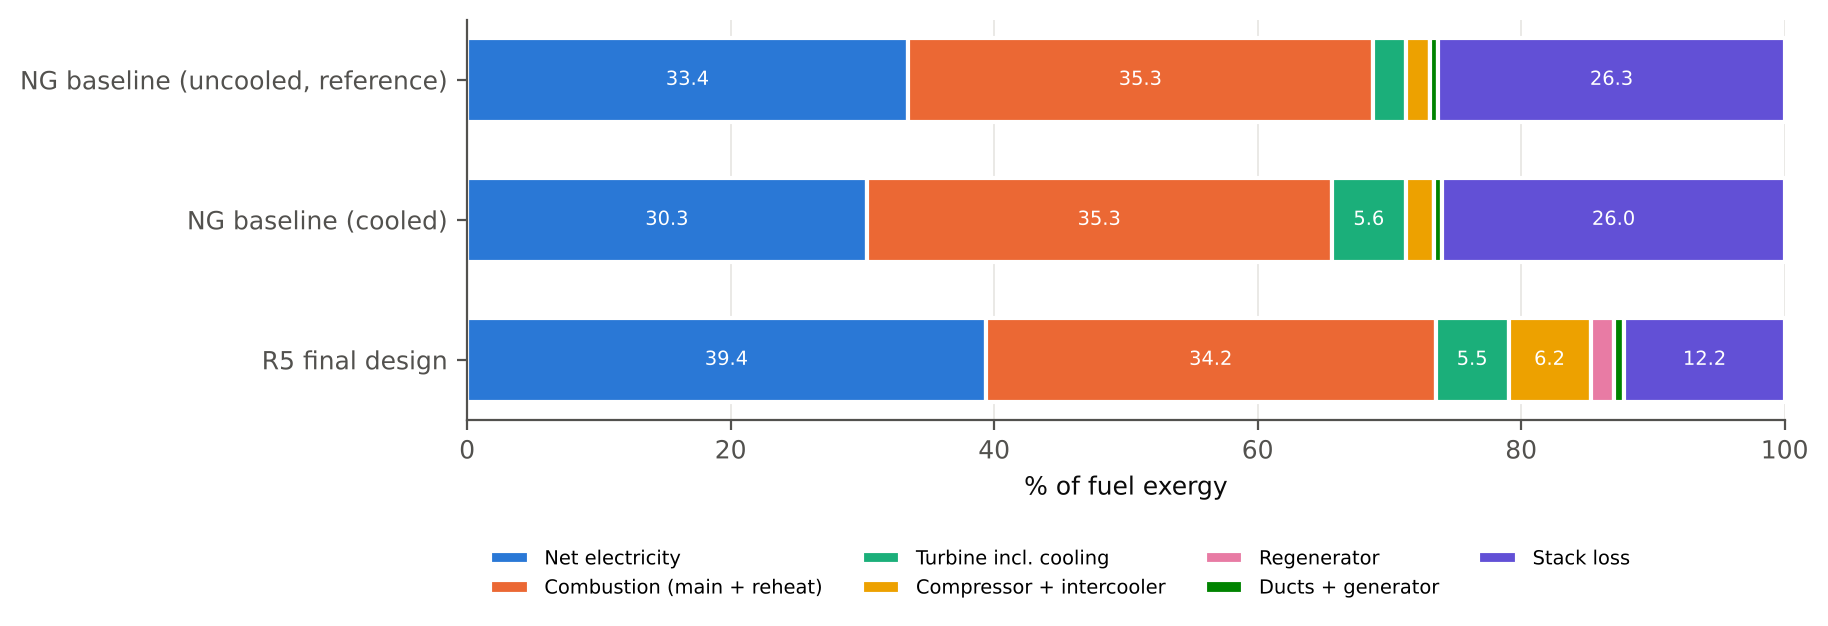
\includegraphics[width=0.9\textwidth]{../figures/fig_exergy_balance.png}
\caption{Where the fuel exergy goes.}\label{fig:ex}\end{figure}
Combustion is the largest loss in every case, about 34--35\% of the fuel exergy. At a fixed TIT it barely moves with hydrogen share (R2 found 30.0\% to 27.7\% from $x$ = 0 to 1), because it is set by the gap between the flame and the 1673\,K that the cycle can use. The final design raises $\Psi$ from 30.3\% (cooled baseline) to \finPsi\%. The gain comes mainly from halving the stack loss (26.0\%\,$\rightarrow$\,12.2\%) through regeneration. The new irreversibilities this adds are small: intercooler 3.4\% (heat rejected to ambient, R1's convention), regenerator 1.8\%, and slightly more compressor loss.

%=====================================================================
\section{Multi-objective optimisation}\label{sec:moo}
\textbf{Decision variables.} Pressure ratio $r_p\in[8,30]$ (R1). TIT $\in[1300,1500]$\,\textdegree C (R3, web limit). $x\in[0,1]$ by volume (R2). $\varepsilon_{rg}\in[0.50,0.85]$ (R4). Intercooling and reheat on/off (R1, R3) and regeneration on/off give 8 cases. R2's excess-air decision is taken by its re-tuned primary-zone strategy, and R1's intercooler effectiveness is fixed at 0.85.

\textbf{Objectives.} (1) maximise $\eta_{net}$; (2) minimise total exergy destruction (MJ/kWh); (3) minimise LCOE; (4) minimise direct CO$_2$ (green H$_2$, zero upstream); (5) minimise the NOx index.

\textbf{Constraints.} NOx $\le$ 75\,ppm; $FI\le2.0$; combustor inlet $\le1050$\,K; reheat-combustor H$_2$ autoignition limit; regenerator only if $T_4>T_2$ with $\ge$20\,K approaches; TIT $\le$ 1500\,\textdegree C (bound). Cooling feasibility ($\phi<0.98$) is also checked.

\textbf{Method.} NSGA-II [Deb 2002] was written in NumPy, because pymoo was not available in the build environment. It uses constrained domination, SBX crossover ($\eta$=15, $p_c$=0.9), polynomial mutation ($\eta$=20, $p_m=1/n$), and population 100 for 150 generations per configuration (8 runs, 120,800 evaluations). A structured grid scan ($r_p$ 8--30 step 2 $\times$ 5 TITs $\times$ 11 blends $\times$ 4 effectivenesses) supplies the constraint-filtering statistics. The feasible designs from both were merged and filtered to the global 5-objective non-dominated set.

\begin{table}[H]\centering\small\caption{Constraint filtering on the grid scan, and Pareto membership by configuration.}\label{tab:feas}
\begin{tabular}{lrr}\toprule Constraint & Designs violating & Violating only this one\\\midrule
NOx > CPCB 75 ppm & 3,354 & 1,245\\
flashback index > 2.0 & 5,234 & 1,216\\
combustor inlet > 1050 K & 1,038 & 253\\
reheat-combustor H$_2$ autoignition & 3,900 & 740\\
regenerator approach < 20 K & 1,415 & 608\\
TIT > firing limit & 0 & 0\\
\midrule Feasible / total & \multicolumn{2}{r}{4,337 / 13,200}\\
\bottomrule\end{tabular}\\[6pt]
\begin{tabular}{lrrr}\toprule Configuration & Feasible & Scanned & Pareto members\\\midrule
Simple & 309 & 660 & 0\\
Reheat & 218 & 660 & 0\\
Regen & 494 & 2,640 & 0\\
Regen+Reheat & 702 & 2,640 & 0\\
IC & 336 & 660 & 304\\
IC+Reheat & 240 & 660 & 906\\
IC+Regen & 1,270 & 2,640 & 3,845\\
IC+Regen+Reheat & 768 & 2,640 & 4,598\\
\bottomrule\end{tabular}
\end{table}
\begin{figure}[H]\centering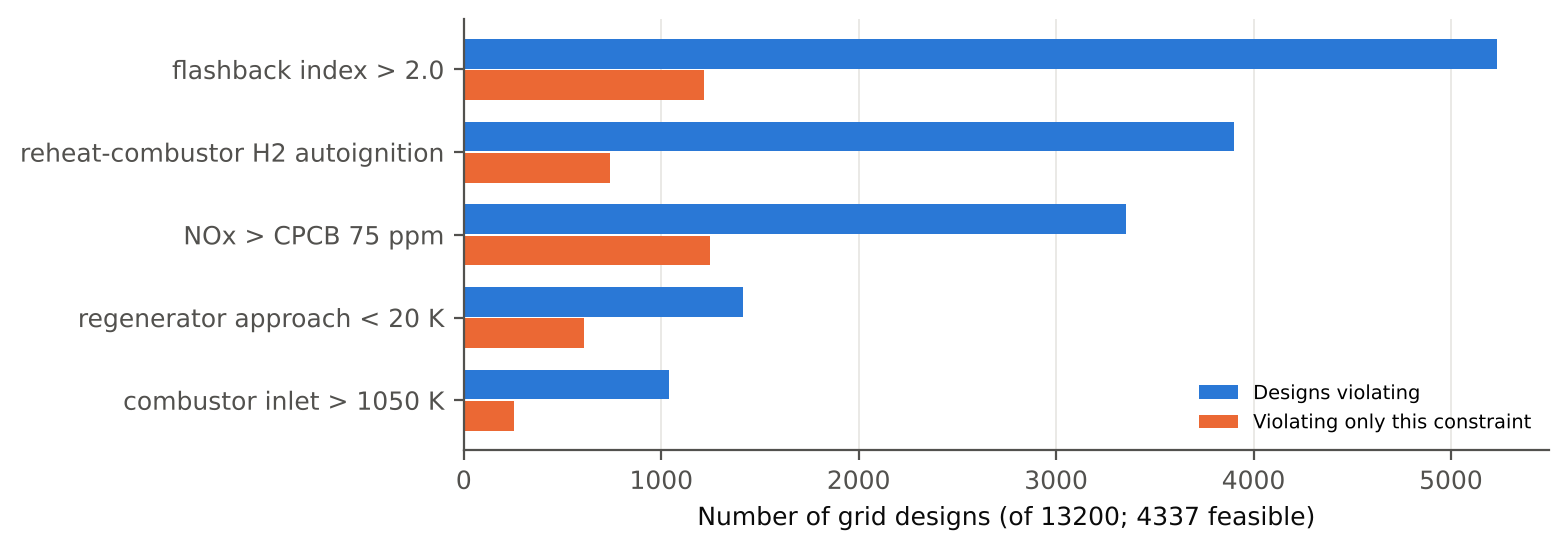
\includegraphics[width=0.7\textwidth]{../figures/fig_feasibility.png}
\caption{Designs removed by each constraint. TIT never binds, because it is a search bound.}\end{figure}
Flashback removes the most designs (the high-$x$ premixed blends), followed by the reheat autoignition limit and NOx. Only four layouts reach the 5-objective Pareto set, and all four are intercooled. Simple, Regen, Reheat and Regen+Reheat are each dominated by their intercooled counterparts.

\begin{figure}[H]\centering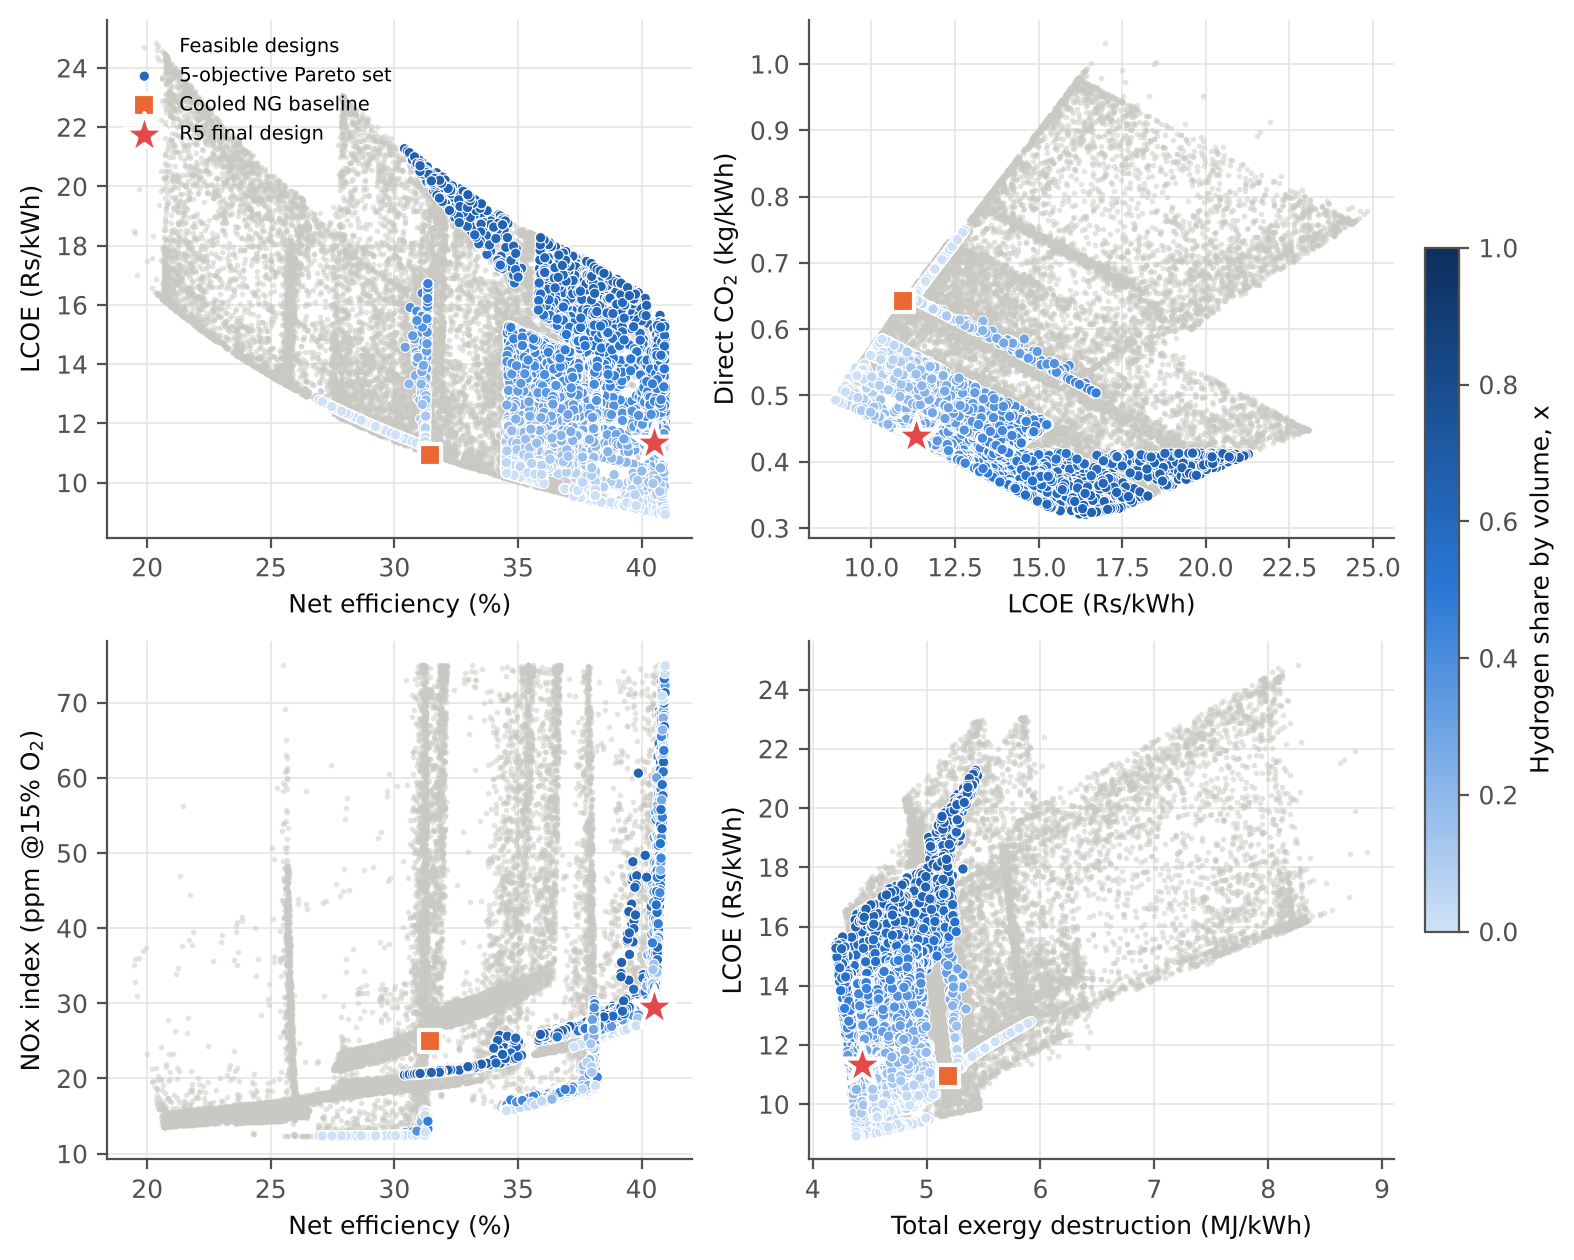
\includegraphics[width=\textwidth]{../figures/fig_pareto_fronts.png}
\caption{Pareto deliverables: efficiency--LCOE, LCOE--CO$_2$, efficiency--NOx and exergy destruction--LCOE. Grey: feasible designs (sample). Coloured: 5-objective Pareto set, shaded by hydrogen share. Square: cooled NG baseline. Star: final design.}\label{fig:pareto}\end{figure}
\textbf{Reading the fronts.} LCOE against CO$_2$ is the sharpest conflict. Along the front, every step of hydrogen buys CO$_2$ at an almost constant price, because fuel cost is linear in energy share. Efficiency against LCOE is not a conflict for $x$ fixed: the high-efficiency IC+Regen designs are also the cheapest. Efficiency against NOx separates the reheat designs (lower NOx, about 38\% efficiency) from the IC+Regen designs (higher NOx, about 40.5\%).

%=====================================================================
\section{Selection of the final design}\label{sec:select}
\subsection{TOPSIS}
TOPSIS was applied to the \nPareto{} Pareto designs with five weight sets and two normalisations. Vector normalisation is the textbook default; min-max normalisation scales each objective by its range.
\begin{table}[H]\centering\scriptsize\caption{TOPSIS winners. LCOE in Rs/kWh, CO$_2$ in kg/kWh, NOx in ppm.}\label{tab:topsis}
\adjustbox{max width=\textwidth}{\begin{tabular}{llllrrrrrrrr}\toprule Normalisation & Weights & Configuration & PR & TIT (\textdegree C) & $x$ & $\varepsilon$ & $C^*$ & $\eta_{net}$ (\%) & LCOE & CO$_2$ & NOx\\\midrule
vector & Equal weights & IC+Regen+Reheat & 30.0 & 1300 & 0.30 & 0.85 & 0.823 & 37.9 & 12.11 & 0.469 & 18.4\\
vector & Cost-led & IC+Regen+Reheat & 26.0 & 1300 & 0.00 & 0.85 & 0.856 & 38.1 & 9.59 & 0.531 & 18.2\\
vector & Climate-led & IC+Regen+Reheat & 26.6 & 1322 & 0.47 & 0.85 & 0.794 & 38.1 & 14.12 & 0.414 & 19.5\\
vector & Efficiency-led & IC+Regen+Reheat & 26.0 & 1300 & 0.30 & 0.85 & 0.819 & 38.1 & 12.07 & 0.467 & 18.8\\
vector & Safety/NOx-led & IC+Regen+Reheat & 30.0 & 1301 & 0.19 & 0.60 & 0.889 & 35.5 & 11.63 & 0.531 & 16.6\\
\addlinespace
min-max & Equal weights & IC+Regen & 16.0 & 1400 & 0.30 & 0.85 & 0.801 & 40.5 & 11.34 & 0.439 & 29.6\\
min-max & Cost-led & IC+Regen & 14.0 & 1400 & 0.00 & 0.85 & 0.856 & 40.6 & 8.99 & 0.498 & 29.4\\
min-max & Climate-led & IC+Regen & 16.0 & 1400 & 0.60 & 0.85 & 0.831 & 40.6 & 15.28 & 0.338 & 31.4\\
min-max & Efficiency-led & IC+Regen & 14.0 & 1400 & 0.30 & 0.85 & 0.867 & 40.6 & 11.33 & 0.439 & 30.3\\
min-max & Safety/NOx-led & IC+Regen+Reheat & 28.0 & 1400 & 0.30 & 0.85 & 0.829 & 38.0 & 12.07 & 0.468 & 19.2\\
\bottomrule\end{tabular}}
\end{table}
The choice depends on the normalisation, not just the weights. Vector normalisation measures each objective relative to its root-mean-square value over the set. The NOx index varies by a large \emph{relative} amount across the set (12--75\,ppm), so it dominates, and every weight set picks the low-NOx reheat design. With min-max scaling, four of the five weight sets pick IC+Regen.

\subsection{Reasoned trade-off between the two equal-weight winners}
\begin{table}[H]\centering\small\caption{Head-to-head of the two equal-weight TOPSIS winners.}\label{tab:h2h}
\begin{tabular}{lccc}\toprule & A: vector-TOPSIS winner & B: min-max-TOPSIS winner & Better\\\midrule
Configuration & IC+Regen+Reheat & IC+Regen & \\
Pressure ratio & 30 & 16 & \\
TIT (\textdegree C) & 1300 & 1400 & \\
H$_2$ share $x$ (vol.) & 0.30 & 0.30 & \\
Regenerator $\varepsilon$ & 0.85 & 0.85 & \\
Net efficiency (\%) & 37.9 & 40.5 & B\\
Exergy destruction (MJ/kWh) & 4.61 & 4.43 & B\\
LCOE (Rs/kWh) & 12.11 & 11.34 & B\\
Direct CO$_2$ (kg/kWh) & 0.469 & 0.439 & B\\
NOx index (ppm) & 18.4 & 29.6 & A\\
\bottomrule\end{tabular}
\end{table}
Design B is chosen. The decision rule was fixed in the code before reading the result: \emph{prefer the candidate that is better on the majority of objectives, provided its NOx keeps at least a one-third margin to the CPCB limit ($\le50$\,ppm)}. The reasons are:
\begin{enumerate}[leftmargin=1.4em,itemsep=1pt]
\item B is better on 4 of 5 objectives: +2.6 points of efficiency, $-$0.18\,MJ/kWh exergy destruction, $-$\Rs0.77/kWh and $-$6\% CO$_2$.
\item A's only advantage is an 11\,ppm lower NOx \emph{index}. This index is calibrated to an assumed 25\,ppm anchor and is a relative measure (R2). B, at \finNOx\,ppm, is under the 50\,ppm band as well as the 75\,ppm limit.
\item B has no reheat combustor. That avoids its autoignition-stabilised operation, whose hydrogen tolerance (R2: $x\le0.41$ at PR 15) would have to be extrapolated to PR 30. It also saves \Rs50 crore of hardware and avoids cooling a second turbine.
\item B operates at R1's and R2's validated pressure-ratio range (PR 16) rather than at the PR 30 search bound.
\end{enumerate}
The rounded specification (PR \finPR, TIT \finTITC\,\textdegree C, $x=\finX$, $\varepsilon=\finEps$) was re-evaluated. It is feasible and is dominated by \nDom{} of the \nFeas{} feasible designs. The same choice is made at hydrogen prices of \Rs280, 350 and 400/kg (Table~\ref{tab:robust}).

%=====================================================================
\section{Final design}\label{sec:final}
\begin{table}[H]\centering\small\caption{State points of the final design (100\,MW net).}\label{tab:states}
\begin{tabular}{cllll}\toprule State & Location & $T$ (K) & $p$ (bar) & $\dot m$ (kg/s)\\\midrule
0 & Ambient & 308.1 & 1.013 & --\\
1 & Compressor inlet (after 1\% loss) & 308.1 & 1.003 & 237.6\\
1a & LP compressor exit & 481.8 & 4.052 & 237.6\\
1b & Intercooler exit & 334.2 & 3.971 & 237.6\\
2 & HP compressor exit / coolant bleed & 522.5 & 16.046 & 237.6\\
5 & Regenerator air out = combustor inlet & 825.6 & 15.725 & 213.2\\
3 & Combustor exit = turbine inlet & 1673.2 & 15.096 & 218.0\\
4 & Turbine exit (after coolant mixing) & 879.1 & 1.044 & 242.4\\
6 & Regenerator gas out & 647.1 & 1.023 & 242.4\\
7 & Stack & 647.1 & 1.013 & 242.4\\
\bottomrule\end{tabular}
\end{table}
\begin{table}[H]\centering\small\caption{Final design against the baselines and against the same cycle on natural gas only.}\label{tab:perf}
\begin{tabular}{lrrrr}\toprule & NG baseline & NG baseline & Final cycle & \textbf{R5 final}\\ & (plan, uncooled) & (cooled) & on NG only & \textbf{design}\\\midrule
Configuration & Simple & Simple & IC+Regen & \textbf{IC+Regen}\\
Pressure ratio & 15 & 15 & 16 & \textbf{16}\\
TIT (\textdegree C) & 1400 & 1400 & 1400 & \textbf{1400}\\
H$_2$ share $x$ (energy share) & 0.00 (0.0\%) & 0.00 (0.0\%) & 0.00 (0.0\%) & \textbf{0.30 (11.9\%)}\\
Regenerator $\varepsilon$ & -- & -- & 0.85 & \textbf{0.85}\\
Blade coolant (\% of air) & 0.0 & 15.0 & 10.2 & \textbf{10.3}\\
Net work (kJ/kg air) & 444 & 342 & 425 & \textbf{427}\\
Cycle efficiency (\%) & 35.2 & 31.9 & 41.1 & \textbf{41.1}\\
Net efficiency (\%) & 34.7 & 31.4 & 40.5 & \textbf{40.5}\\
Heat rate (kJ/kWh) & 10,384 & 11,454 & 8,892 & \textbf{8,885}\\
Air flow (kg/s) & 228.6 & 296.5 & 239.0 & \textbf{237.6}\\
Fuel flow (kg/s) & 6.01 & 6.63 & 5.15 & \textbf{4.78}\\
of which H$_2$ (kg/s) & 0.000 & 0.000 & 0.000 & \textbf{0.244}\\
Combustor inlet $T_5$ (K) & 722 & 722 & 826 & \textbf{826}\\
Stack $T$ (K) & 945 & 876 & 647 & \textbf{647}\\
Exergy destruction (MJ/kWh) & 4.34 & 5.19 & 4.50 & \textbf{4.43}\\
Second-law efficiency $\Psi$ (\%) & 33.4 & 30.3 & 39.1 & \textbf{39.4}\\
Capital cost (Rs crore) & 400 & 400 & 480 & \textbf{534}\\
LCOE (Rs/kWh) & 10.03 & 10.94 & 9.00 & \textbf{11.34}\\
Direct CO$_2$ (kg/kWh) & 0.583 & 0.643 & 0.499 & \textbf{0.439}\\
NOx index (ppm @15\% O$_2$) & 25.0 & 25.0 & 28.7 & \textbf{29.6}\\
Flashback index (--) & 1.00 & 1.00 & 1.00 & \textbf{1.29}\\
\bottomrule\end{tabular}
\end{table}
\begin{table}[H]\centering\small\caption{Capital cost of the final design.}\label{tab:capex}
\begin{tabular}{lrl}\toprule Capital item & Rs crore & Basis\\\midrule
base plant & 400.0 & Rs 4 cr/MW [PS]\\
hot section (TIT) & 0.0 & +4\%/100 K above 1400\textdegree C [R3]\\
intercooler & 26.0 & 6.5\% of base [R1]\\
regenerator & 53.6 & $\propto UA$, Rs 40 cr at $UA$ = 576 kW/K [R4]\\
reheat & 0.0 & 12.5\% of base [R3]\\
H$_2$ combustor premium & 16.0 & 0--4--15\% of base vs $x$ [R2]\\
H$_2$ storage & 38.7 & 8 h full-load H$_2$ at Rs 55,000/kg [R2]\\
\midrule Total & 534.3 & \\\bottomrule\end{tabular}
\end{table}
\begin{table}[H]\centering\small\caption{LCOE build-up (hydrogen supply in the fuel line, storage separate).}\label{tab:lcoe}
\begin{tabular}{lrrr}\toprule Rs/kWh & NG baseline (plan) & NG baseline (cooled) & R5 final design\\\midrule
capital recovery & 0.93 & 0.93 & 1.15\\
O\&M & 0.27 & 0.27 & 0.34\\
H$_2$ storage & 0.00 & 0.00 & 0.12\\
fuel & 8.83 & 9.74 & 9.73\\
\midrule LCOE & 10.03 & 10.94 & 11.34\\
Direct CO$_2$ (kg/kWh) & 0.583 & 0.643 & 0.439\\\bottomrule\end{tabular}
\end{table}
\textbf{Operating point.} The final design needs \finMair\,kg/s of air and \finMfuel\,kg/s of blended fuel, of which \finMh\,kg/s is hydrogen. Eight hours of storage holds \finStore\,t of H$_2$. The regenerator recovers \finQrg\,MW, raising combustor air to \finTfive\,K (well below the 1050\,K autoignition limit) and cooling the stack to \finTsix\,K. It needs about \finArea\,m$^2$ of surface at $U=50$\,W/m$^2$K. The flashback index is \finFI, within a tier-B premixer. Fuel is \fuelShare\% of the LCOE.

\textbf{CO$_2$ cost.} Against the cooled baseline, the design cuts direct CO$_2$ by \dCOpct\% for +\dLpct\% LCOE, an average of \Rs\abateTot{} per tonne avoided. This splits into two very different parts:
\begin{itemize}[leftmargin=1.2em,itemsep=1pt]
\item The cycle improvement (same cycle on natural gas: \ngCO\,kg/kWh, \Rs\ngLCOE/kWh) gives $-$\dCOcyclepct\% CO$_2$ at a \emph{negative} cost (\Rs\abateCycle/t). It saves money.
\item The 30\% hydrogen blend adds the rest at about \Rs\abateHtwo/t, consistent with R2's \Rs36,000--44,000/t.
\end{itemize}
Efficiency is the cheap decarbonisation lever, and hydrogen the expensive one.

%=====================================================================
\section{What the final design gives up against each role's best}\label{sec:roles}
\begin{table}[H]\centering\scriptsize\caption{Each role's individually-best value within the feasible set, against the final design.}\label{tab:roles}
\adjustbox{max width=\textwidth}{\begin{tabular}{p{2.6cm}p{3.6cm}rp{5.2cm}r}\toprule Role & Metric & Role-best & Design achieving it & Final design\\\midrule
R1 Compressor \& IC & Compressor + intercooler exergy destruction (\% fuel exergy) & 1.2 & Reheat, PR 8.0, TIT 1450 C, x 0.00 & 6.2\\
R2 Combustor \& blend & NOx index (ppm) & 12.4 & IC+Reheat, PR 11.6, TIT 1400 C, x 0.00 & 29.6\\
R2 Combustor \& blend & Combustion exergy destruction (all combustors) (\% fuel exergy) & 29.2 & Regen+Reheat, PR 19.7, TIT 1466 C, x 0.42, eps 0.71 & 34.2\\
R3 Turbine \& reheat & Specific net work (machine size) (kJ/kg air) & 580 & IC+Reheat, PR 30.0, TIT 1497 C, x 0.47 & 427\\
R3 Turbine \& reheat & Turbine exergy destruction incl. cooling (\% fuel exergy) & 3.1 & IC, PR 8.0, TIT 1300 C, x 0.00 & 5.5\\
R4 Regenerator & Stack exergy loss (\% fuel exergy) & 11.6 & IC+Regen, PR 22.0, TIT 1300 C, x 0.00, eps 0.85 & 12.2\\
R5 Integration & Net efficiency (\%) & 41.0 & IC+Regen, PR 14.6, TIT 1447 C, x 0.47, eps 0.85 & 40.5\\
R5 Integration & Total exergy destruction (MJ/kWh) & 4.20 & IC+Regen, PR 13.2, TIT 1444 C, x 0.61, eps 0.85 & 4.43\\
R5 Integration & LCOE (Rs/kWh) & 8.93 & IC+Regen, PR 14.8, TIT 1450 C, x 0.00, eps 0.85 & 11.34\\
R5 Integration & Direct CO$_2$ (kg/kWh) & 0.321 & IC+Regen, PR 22.1, TIT 1438 C, x 0.65, eps 0.79 & 0.439\\
\bottomrule\end{tabular}}
\end{table}
\begin{itemize}[leftmargin=1.2em,itemsep=1pt]
\item \textbf{R1.} Intercooling adds 3.4\% of fuel exergy as rejected heat, so R1's component destruction (6.2\%) is far above its best (1.2\%, a low-PR non-intercooled design). The system gains are lower coolant and a wider regeneration margin, which more than repay it. R1's intercooler candidate ($\varepsilon=0.85$) is adopted unchanged.
\item \textbf{R2.} NOx 29.6 against the best 12.4\,ppm (IC+Reheat on natural gas). The hydrogen share of 0.30 is below R2's stand-in 0.40 and far below R2's climate optimum ($x=1$, which is infeasible on flashback). At \Rs350/kg the 5-objective trade-off does not justify more hydrogen.
\item \textbf{R3.} TIT stays at 1400\,\textdegree C rather than R3's maximum-efficiency 1500\,\textdegree C. With cooling the efficiency gain is small, and with R2's primary-zone margin NOx exceeds 75\,ppm above about 1450\,\textdegree C. Reheat is not used, which gives up R3's maximum specific work (580 against 427\,kJ/kg): a 36\% larger air flow is the price.
\item \textbf{R4.} $\varepsilon=0.85$ is R4's upper screening bound. The stack loss of 12.2\% is close to R4's best of 11.6\%.
\item \textbf{R5.} Efficiency is within 0.5 points of the best feasible. LCOE is \Rs2.4/kWh above the cheapest feasible design (IC+Regen on natural gas), which is the price of the hydrogen blend.
\end{itemize}
\begin{table}[H]\centering\scriptsize\caption{Each teammate's submitted candidate re-run through the cooled integrated model.}\label{tab:rolecands}
\adjustbox{max width=\textwidth}{\begin{tabular}{p{5.0cm}rrrrrp{3.2cm}}\toprule Case (run through the cooled integrated model) & $\eta_{net}$ (\%) & LCOE & CO$_2$ & NOx & FI & Constraint violations\\\midrule
R1 candidate: IC, PR 15, NG & 32.3 & 10.76 & 0.625 & 19.1 & 1.00 & none\\
R2 stand-in: IC+Regen+Reheat, PR 15, x 0.40 & 35.5 & 14.01 & 0.471 & 20.4 & 1.56 & none\\
R3 best: simple, TIT 1500 C, NG & 31.7 & 10.89 & 0.636 & 151.6 & 1.00 & NOx > CPCB 75 ppm\\
R4 candidate: Regen eps 0.75, PR 15, NG & 33.9 & 10.34 & 0.595 & 29.3 & 1.00 & none\\
Cooled NG baseline & 31.4 & 10.94 & 0.643 & 25.0 & 1.00 & none\\
R5 final design & 40.5 & 11.34 & 0.439 & 29.6 & 1.29 & none\\
\bottomrule\end{tabular}}
\end{table}
R3's maximum-efficiency case (simple cycle, 1500\,\textdegree C) breaks the NOx limit once the primary-zone temperature follows TIT. R2's uncooled stand-in loses 8 points of efficiency once both of its turbines are cooled.

%=====================================================================
\section{Sensitivity and robustness}\label{sec:sens}
\begin{figure}[H]\centering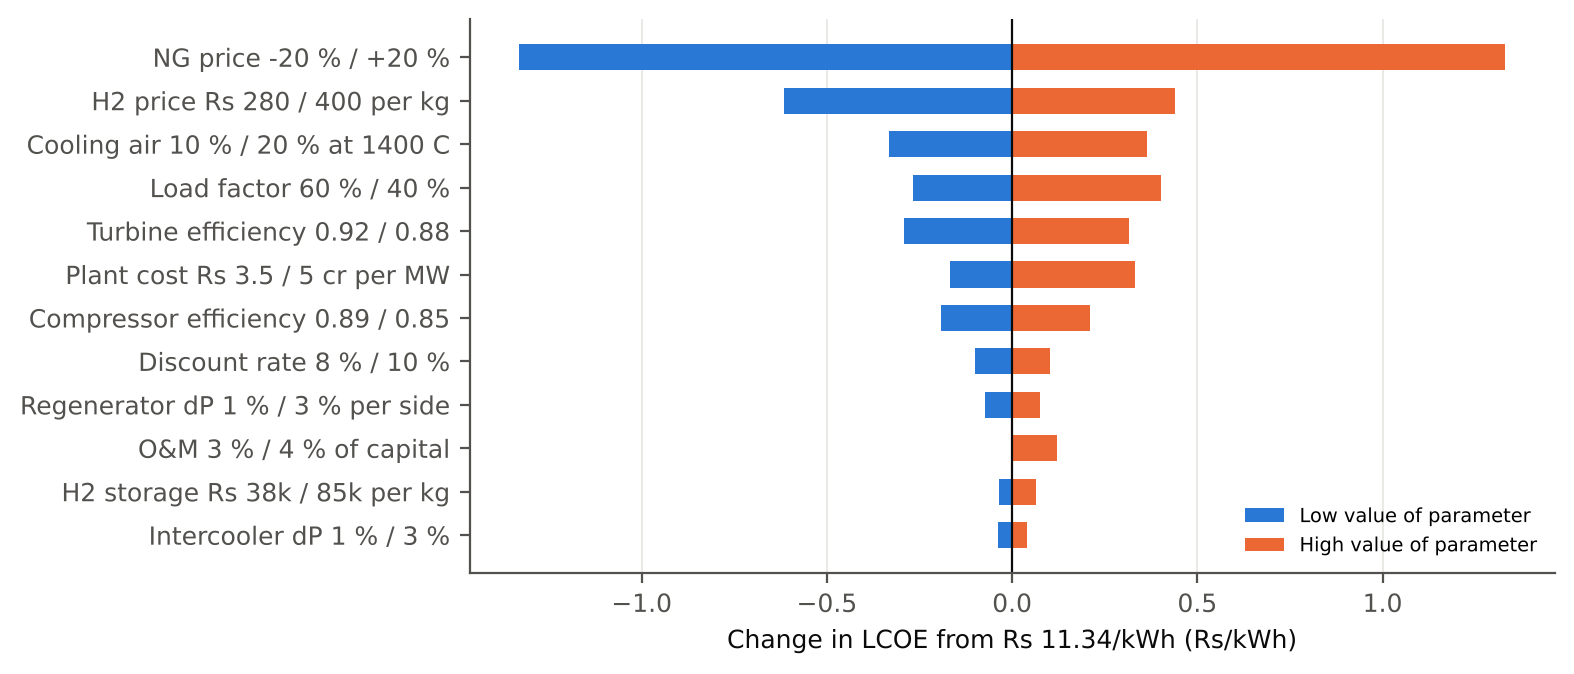
\includegraphics[width=0.75\textwidth]{../figures/fig_tornado.png}
\caption{One-at-a-time sensitivity of the final design's LCOE.}\label{fig:tornado}\end{figure}
\begin{table}[H]\centering\scriptsize\caption{Sensitivity of the final design. It stays feasible in every case.}\label{tab:sens}
\begin{tabular}{lrrrrrr}\toprule Parameter (low / high) & \multicolumn{2}{c}{LCOE (Rs/kWh)} & \multicolumn{2}{c}{$\eta_{net}$ (\%)} & \multicolumn{2}{c}{CO$_2$ (kg/kWh)}\\ & low & high & low & high & low & high\\\midrule
NG price -20 \% / +20 \% & 10.01 & 12.67 & 40.5 & 40.5 & 0.439 & 0.439\\
H$_2$ price Rs 280 / 400 per kg & 10.72 & 11.78 & 40.5 & 40.5 & 0.439 & 0.439\\
Cooling air 10 \% / 20 \% at 1400 C & 11.01 & 11.70 & 42.0 & 39.1 & 0.424 & 0.456\\
Load factor 60 \% / 40 \% & 11.07 & 11.74 & 40.5 & 40.5 & 0.439 & 0.439\\
Turbine efficiency 0.92 / 0.88 & 11.05 & 11.66 & 41.7 & 39.3 & 0.427 & 0.453\\
Plant cost Rs 3.5 / 5 cr per MW & 11.17 & 11.67 & 40.5 & 40.5 & 0.439 & 0.439\\
Compressor efficiency 0.89 / 0.85 & 11.15 & 11.55 & 41.3 & 39.7 & 0.431 & 0.449\\
Discount rate 8 \% / 10 \% & 11.24 & 11.44 & 40.5 & 40.5 & 0.439 & 0.439\\
Regenerator dP 1 \% / 3 \% per side & 11.27 & 11.41 & 40.8 & 40.2 & 0.436 & 0.443\\
O\&M 3 \% / 4 \% of capital & 11.34 & 11.46 & 40.5 & 40.5 & 0.439 & 0.439\\
H$_2$ storage Rs 38k / 85k per kg & 11.30 & 11.40 & 40.5 & 40.5 & 0.439 & 0.439\\
Intercooler dP 1 \% / 3 \% & 11.30 & 11.38 & 40.7 & 40.4 & 0.438 & 0.441\\
\bottomrule\end{tabular}
\end{table}
\begin{figure}[H]\centering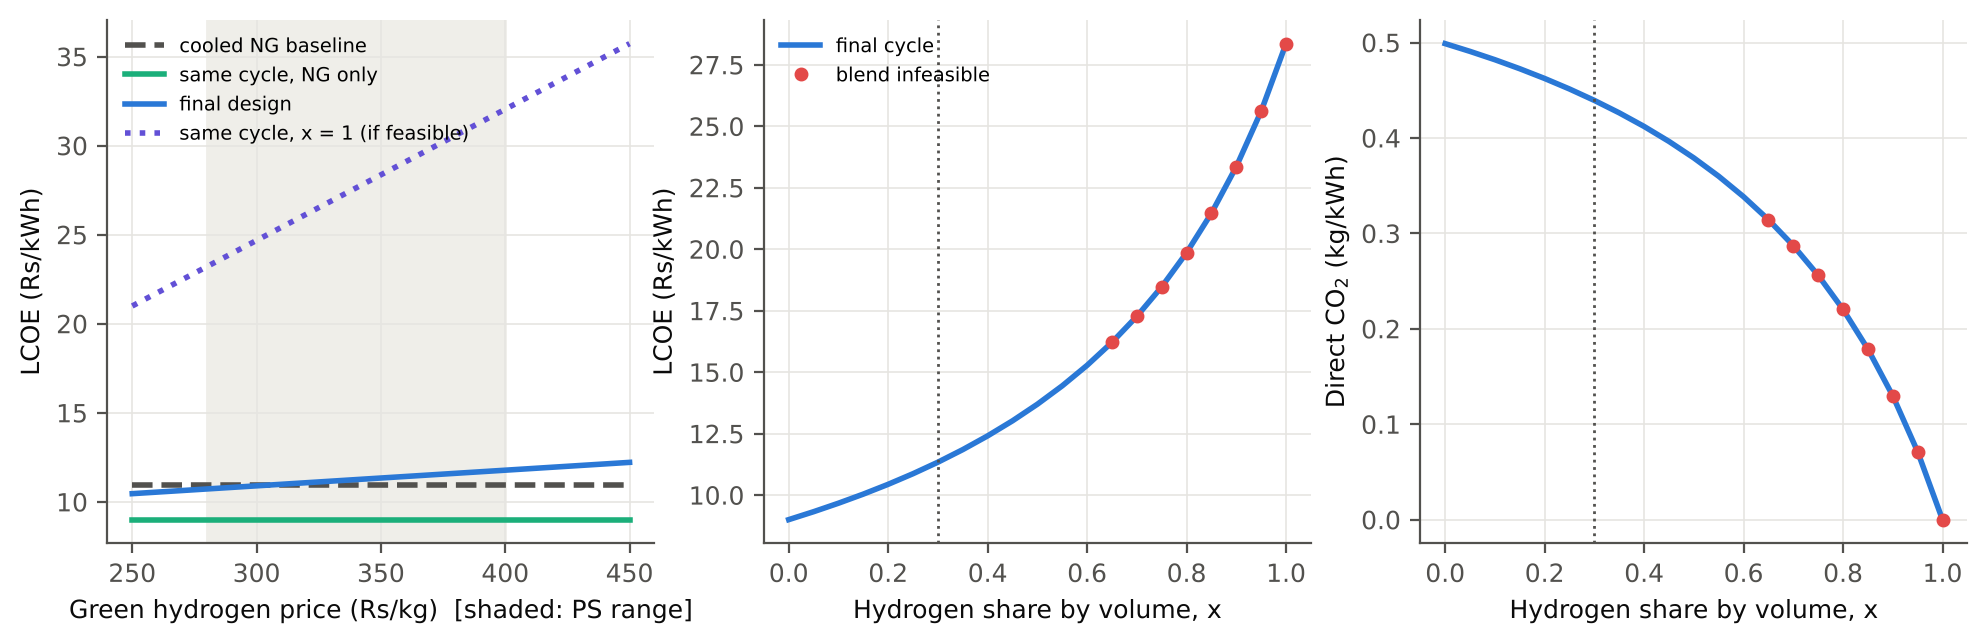
\includegraphics[width=\textwidth]{../figures/fig_h2_price_share.png}
\caption{Left: LCOE against hydrogen price. Centre and right: LCOE and CO$_2$ against hydrogen share on the final cycle. Red dots mark blends that break the flashback limit ($x\ge0.65$).}\label{fig:h2}\end{figure}
\begin{table}[H]\centering\small\caption{Robustness of the selection to hydrogen price (equal weights).}\label{tab:robust}
\begin{tabular}{rllrrrrr}\toprule H$_2$ price (Rs/kg) & Normalisation & Configuration & PR & TIT (\textdegree C) & $x$ & $\varepsilon$ & LCOE\\\midrule
280 & vector & IC+Regen+Reheat & 30 & 1300 & 0.30 & 0.85 & 11.45\\
280 & min-max & IC+Regen & 16 & 1400 & 0.30 & 0.85 & 10.72\\
350 & vector & IC+Regen+Reheat & 30 & 1300 & 0.30 & 0.85 & 12.11\\
350 & min-max & IC+Regen & 16 & 1400 & 0.30 & 0.85 & 11.34\\
400 & vector & IC+Regen+Reheat & 30 & 1300 & 0.20 & 0.85 & 11.44\\
400 & min-max & IC+Regen & 16 & 1400 & 0.30 & 0.85 & 11.78\\
\bottomrule\end{tabular}
\end{table}
The natural-gas price (fuel is \fuelShare\% of LCOE) and the hydrogen price dominate. Across the problem statement's H$_2$ range of \Rs280--400/kg, LCOE moves from \Rs\lcoeLo{} to \Rs\lcoeHi/kWh. Of the engineering assumptions, the cooling-air fraction and the turbine efficiency matter most (about $\pm$1.5 points of efficiency). The exchanger pressure losses matter little. The configuration, PR, TIT, $x$ and $\varepsilon$ do not change across the hydrogen-price range.

%=====================================================================
\section{Limitations}\label{sec:lim}
\begin{itemize}[leftmargin=1.2em,itemsep=1pt]
\item \textbf{Constant-$c_p$ model} (plan requirement). Hydrogen enters only through R2's tabulated $c_{p,g}$ and $\gamma_g$. R2 found that this overstates fuel use by about 2.4\% against Cantera.
\item \textbf{Cooling model and data} are semi-empirical, calibrated by assumption to 15\% coolant at 1400\,\textdegree C. Coolant is throttled from compressor delivery for both turbines. Real reheat machines feed the LP turbine with lower-pressure bleed and fire it below TIT, which would soften the reheat penalty.
\item \textbf{The NOx index} is calibrated, not predicted, and so is the primary-zone margin rule above 1400\,\textdegree C. The NOx surrogate (inlet temperature, reheat dilution) is fitted to R2's eight points at $x=0$. The CPCB limit still needs checking against the Gazette.
\item \textbf{Capital costs} are the problem statement's percentage allowances, with no scale credit for smaller machines (high specific work). Storage cost comes from US DOE onboard-tank figures, and O\&M is held at 3\% for hydrogen.
\item \textbf{Fixed choices.} Intercooler $\varepsilon$ is fixed at 0.85, and exchanger losses at 2\%. The reheat split is fixed and reheat fires to TIT. TOPSIS weights are judgements; the selection was checked across 10 weight/normalisation combinations.
\item Direct CO$_2$ only. Green H$_2$ is assumed to have zero upstream emissions; grey H$_2$ would remove the CO$_2$ benefit of the blend.
\end{itemize}

%=====================================================================
\section{Conclusions}
\begin{enumerate}[leftmargin=1.4em,itemsep=2pt]
\item The integrated model reproduces the plan's reference baseline and all R1--R4 hand-offs, and its exergy balance closes.
\item Adding blade cooling (web-sourced data) changes the ranking. Reheat, favoured by R2's uncooled screening, is penalised. Intercooled regeneration becomes the best layout because it cuts both the coolant demand and the stack loss.
\item \textbf{Recommended design: IC + regeneration, PR \finPR, TIT \finTITC\,\textdegree C, $x=\finX$ by volume (\finE\% energy), $\varepsilon_{rg}=\finEps$.} It achieves $\eta_{net}=\finEta\%$, heat rate \finHR\,kJ/kWh, $\Psi=\finPsi\%$, LCOE \Rs\finLCOE/kWh, \finCO\,kg CO$_2$/kWh and NOx index \finNOx\,ppm, and satisfies every constraint with margin.
\item Against the cooled natural-gas baseline, CO$_2$ falls by \dCOpct\% for a \dLpct\% higher LCOE. Most of the CO$_2$ cut comes from efficiency, at negative cost. The hydrogen part costs about \Rs\abateHtwo/t, so deeper blending waits on cheaper hydrogen and on flashback-proof burners for $x>0.65$.
\end{enumerate}

\section*{References}
\small
\begin{itemize}[leftmargin=1.2em,itemsep=0pt]
\item[{[PS]}] Problem 16 -- Full problem statement; Problem 16 -- Four-week team plan (supplied).
\item[{[R1--R4]}] Team submissions: R1 Compressor \& intercooling; R2 Combustor \& fuel blend (incl.\ its references: Heywood; Lefebvre \& Ballal; Lewis \& von Elbe; Szargut; GRI-Mech 3.0; US DOE storage record 13010); R3 Turbine \& reheat (report and code); R4 Regenerator, Part A.
\item[{[W1]}] Mitsubishi Heavy Industries, \emph{Technical Review} Vol.\,56 No.\,3 (2019): development of the 1650\,\textdegree C-class JAC gas turbine (F-series 1350--1400\,\textdegree C, G/H-series 1500\,\textdegree C, J-series 1600\,\textdegree C). \url{https://power.mhi.com/randd/technical-review/pdf/index_67e.pdf}
\item[{[W2]}] Hada S., Takata K., ``High-efficiency gas turbine development applying 1600\,\textdegree C class J technology'', MHI Technical Review. \url{https://power.mhi.com/randd/technical-review/pdf/index_20e.pdf}
\item[{[W3]}] University of Cambridge, Phase Transformations group, ``Coatings for turbine blades''. \url{https://www.phase-trans.msm.cam.ac.uk/2003/Superalloys/coatings/}
\item[{[W4]}] Harris K., Erickson G.L. et al., Cannon-Muskegon Corp., CMSX-4 single-crystal superalloy turbine blades (ASME paper). \url{https://core.ac.uk/download/357389784.pdf}
\item[{[W5]}] ASME J.\ Eng.\ Gas Turbines Power 10.1115/1.4048452 and related abstracts (blade cooling air about 20\% of compressor suction air at 1350\,\textdegree C-class TIT). \url{https://next.sciencegate.app/document/10.1115/1.4048452}
\item[{[W6]}] CEAS Aeronautical Journal (2024), comparison of cooling-air estimation methods (Horlock, Jonsson, Halliwell). \url{https://link.springer.com/article/10.1007/s13272-024-00776-0}
\item[{[Deb 2002]}] Deb K., Pratap A., Agarwal S., Meyarivan T., ``A fast and elitist multiobjective genetic algorithm: NSGA-II'', \emph{IEEE Trans.\ Evol.\ Comput.} 6(2), 2002.
\item[{[Hwang 1981]}] Hwang C.L., Yoon K., \emph{Multiple Attribute Decision Making}, Springer, 1981 (TOPSIS).
\item[{[Horlock]}] Horlock J.H., Watson D.T., Jones T.V., ``Limitations on gas turbine performance imposed by large turbine cooling flows'', \emph{J.\ Eng.\ Gas Turbines Power} 123, 2001.
\end{itemize}
\normalsize

\appendix
\section{Assumptions log (R5 additions to R1--R4)}
\begin{table}[H]\centering\small
\begin{tabular}{p{4.2cm}p{4.0cm}p{5.6cm}}\toprule Item & Value & Basis\\\midrule
Firing-temperature limit & 1500\,\textdegree C (1773\,K) & G/H-class air-cooled technology [W1,W2]\\
Blade-metal limit / $\eta_{cool}$ & 1150\,K / 0.70 & R3; consistent with [W3,W4]\\
Coolant calibration $B$ & 0.075 (15\% at 1400\,\textdegree C) & Between R3 (12\%) and [W5] (about 20\% incl.\ sealing)\\
Intercooler / regenerator $\Delta p$ & 2\% / 2\% per side & R5 fixed value; R4's range 1--3\%\\
Primary zone above 1400\,\textdegree C & $T_{pz}=1790+(T_3-1673)$ & Keeps R2's dilution margin\\
NOx surrogate & $k=\noxK\times10^{-3}$/K, $n=\noxN$ & Least squares on R2's configuration table\\
Flashback limit & $FI\le2.0$ & Top of R2's tier B (1.94)\\
Regenerator cost & $\propto UA$; Rs 40 cr at 576\,kW/K & R4 calibration\\
Hot-section cost & +4\% of base per 100\,K above 1400\,\textdegree C & R3\\
H$_2$ storage & Rs 55,000/kg, 8 h & R2 (US DOE)\\
Search bounds & PR 8--30; TIT 1300--1500\,\textdegree C; $\varepsilon$ 0.50--0.85 & Heavy-duty practice; R4 screening range\\\bottomrule
\end{tabular}\end{table}

\section{Code and how to reproduce}
\begin{tabular}{ll}
\texttt{r5\_params.py} & Shared parameter file (every number, with its owner and source)\\
\texttt{r5\_model.py} & Integrated cycle, cooling, constraints, exergy, LCOE and CO$_2$\\
\texttt{r5\_validate.py} & Table~\ref{tab:valid}\\
\texttt{r5\_nsga2.py} & NSGA-II (constrained domination, SBX, polynomial mutation)\\
\texttt{r5\_run\_all.py} & Candidates, sweeps, grid scan, NSGA-II, Pareto set (about 10 min)\\
\texttt{r5\_select.py} & TOPSIS, final design, role trade-offs, exergy, LCOE, sensitivity\\
\texttt{r5\_figures.py}, \texttt{r5\_make\_tables.py} & Figures and the LaTeX tables and numbers used in this report\\
\end{tabular}

Run in order: \texttt{r5\_validate.py}, \texttt{r5\_run\_all.py}, \texttt{r5\_select.py}, \texttt{r5\_figures.py}, \texttt{r5\_make\_tables.py} (each with \texttt{python}), then compile this file with \texttt{pdflatex} (twice). Requires Python 3 with NumPy, pandas and matplotlib. The CSV outputs are in \texttt{results/}.
\end{document}
